\section{Introdução}
\label{s.introduction}

\begin{frame}{Introdução}
	\justify 
	\begin{itemize}
		\item<1> A área de Ciência da Computação sempre está evoluindo, onde diariamente dezenas de artigos novos estão disponíveis, e.g., \url{https://arxiv.org};
		\\~\\
		\item<2> Atualmente, centros de pesquisa privados (Microsoft Research, Google Research, OpenAI, etc) estão ``competindo"~diretamente com as universidades;
		\\~\\
		\item<3> Entretanto, como é possível garantir visibilidade, reprodutibilidade e integridade da pesquisa em um mundo altamente competitivo?
	\end{itemize}
\end{frame}


\begin{frame}{}
	\centering
	\begin{figure}
		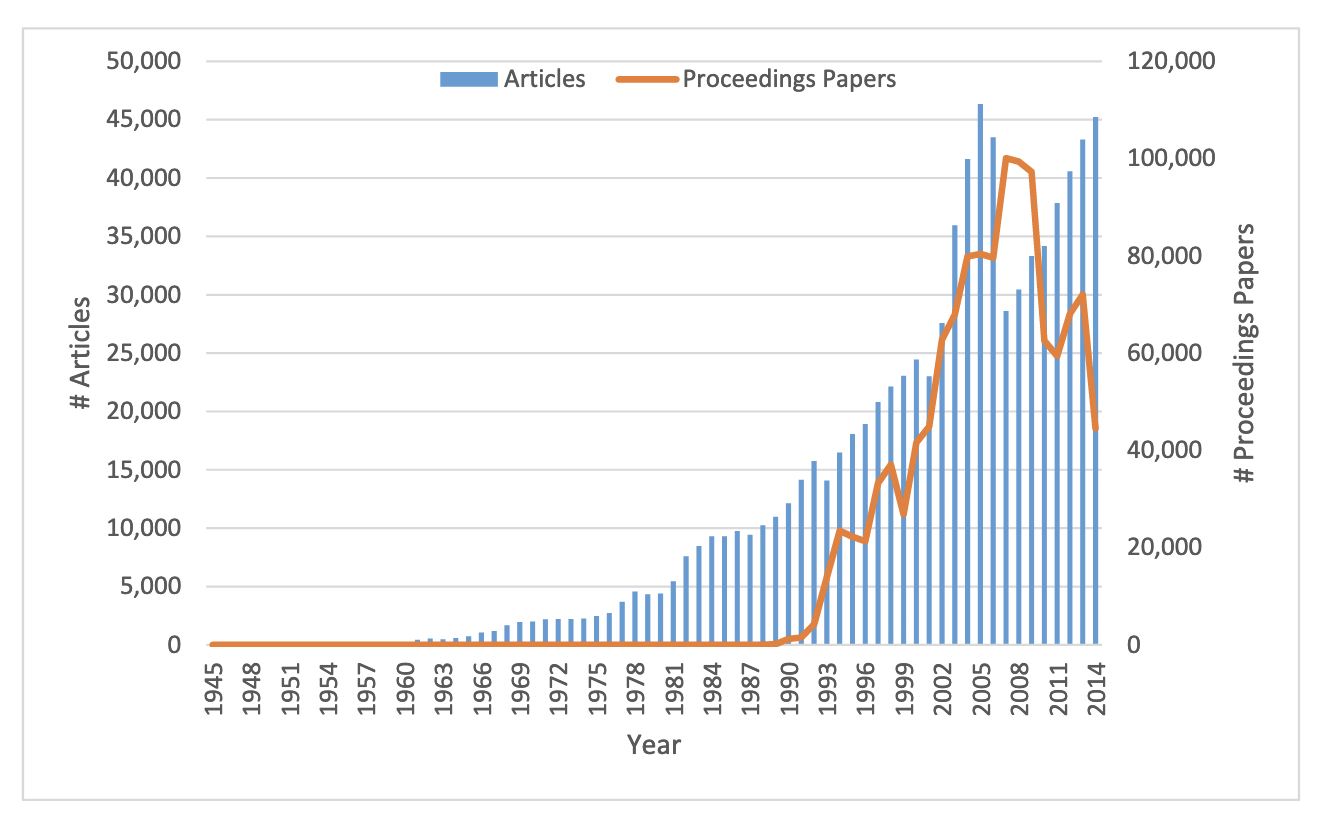
\includegraphics[scale=0.4]{figs/number_of_papers.png}
		\caption{Número de artigos (periódicos em azul e conferências em laranja) publicados em anos individuais~\cite{Fiala:17}.}
		\label{f.number_of_papers}
	\end{figure}	
\end{frame}